\documentclass[a4paper,11pt]{article}

%% packages

\usepackage{blindtext} % needed for creating dummy text passages
%\usepackage{ngerman} % needed for German default language
\usepackage{amsmath} % needed for command eqref
\usepackage{amssymb} % needed for math fonts
\usepackage[colorlinks=true,breaklinks]{hyperref} % needed for creating hyperlinks in the document, the option colorlinks=true gets rid of the awful boxes, breaklinks breaks lonkg links (list of figures), and ngerman sets everything for german as default hyperlinks language
\usepackage[hyphenbreaks]{breakurl} % ben�tigt f�r das Brechen von URLs in Literaturreferenzen, hyphenbreaks auch bei links, die �ber eine Seite gehen (mit hyphenation).
\usepackage{xcolor}
\definecolor{c1}{rgb}{0,0,1} % blue
\definecolor{c2}{rgb}{0,0.3,0.9} % light blue
\definecolor{c3}{rgb}{0.3,0,0.9} % red blue
\hypersetup{
    linkcolor={c1}, % internal links
    citecolor={c2}, % citations
    urlcolor={c3} % external links/urls
}
%\usepackage{cite} % needed for cite
\usepackage[square,authoryear]{natbib} % needed for cite and abbrvnat bibliography style
\usepackage[nottoc]{tocbibind} % needed for displaying bibliography and other in the table of contents
\usepackage{graphicx} % needed for \includegraphics 
\usepackage{longtable} % needed for long tables over pages
\usepackage{bigstrut} % needed for the command \bigstrut
\usepackage{enumerate} % needed for some options in enumerate
%\usepackage{todonotes} % needed for todos
\usepackage{makeidx} % needed for creating an index
\makeindex
\usepackage{gensymb}
\usepackage{url}

%% page settings

\usepackage[top=5mm, bottom=5mm,left=15mm,right=15mm]{geometry} % needed for page border settings
\parindent=0mm % for space of first line of new text block
\sloppy % for writing with hyphenless justification (tries to)
\hyphenation{} % use hyphenation of tolerance parametershttp://www.jr-x.de/publikationen/latex/tipps/zeilenumbruch.html
\hyphenpenalty=10000
\exhyphenpenalty=10000
\usepackage{fancyhdr} % needed for head and foot options
%% my macros

%% Text fomats
\newcommand{\tbi}[1]{\textbf{\textit{#1}}}

%% Math fonts
\newcommand{\bbA}{\mathbb{A}}
\newcommand{\bbB}{\mathbb{B}}
\newcommand{\bbC}{\mathbb{C}}
\newcommand{\bbD}{\mathbb{D}}
\newcommand{\bbE}{\mathbb{E}}
\newcommand{\bbF}{\mathbb{F}}
\newcommand{\bbG}{\mathbb{G}}
\newcommand{\bbH}{\mathbb{H}}
\newcommand{\bbI}{\mathbb{I}}
\newcommand{\bbJ}{\mathbb{J}}
\newcommand{\bbK}{\mathbb{K}}
\newcommand{\bbL}{\mathbb{L}}
\newcommand{\bbM}{\mathbb{M}}
\newcommand{\bbN}{\mathbb{N}}
\newcommand{\bbO}{\mathbb{O}}
\newcommand{\bbP}{\mathbb{P}}
\newcommand{\bbQ}{\mathbb{Q}}
\newcommand{\bbR}{\mathbb{R}}
\newcommand{\bbS}{\mathbb{S}}
\newcommand{\bbT}{\mathbb{T}}
\newcommand{\bbU}{\mathbb{U}}
\newcommand{\bbV}{\mathbb{V}}
\newcommand{\bbW}{\mathbb{W}}
\newcommand{\bbX}{\mathbb{X}}
\newcommand{\bbY}{\mathbb{Y}}
\newcommand{\bbZ}{\mathbb{Z}}
\usepackage{float}
\begin{document}

	Thalagala B.P. 180631J
\begin{center}
{	\Large\textbf{Home Work : Transport Layer}}\\[2mm]

\textbf{December 15, 2021}
\end{center}
\vspace{5mm}
\hrule
\vspace{5mm}
\subsection*{1. Why are transport layer services called end-to-end?}

Transport layer provides a reliable logical connection between two application processes run in two end stations which is achieved through the  protocols implemented inside the Operating Systems. These protocols make sure that the data communication between two application processes reside in two end stations happens in such a way that the relationship among data packets of a given application instance is preserved even though all the applications use a common network interface to send data packets. Port number is used to distinguish different processes of a given host.

\subsection*{2. How do transport layer services differ from network layer services?}

Network layer provides host-to-host reliable communication. Regardless of the processes which packets belong, network layer ensures that each packet reaches from its point of origin to its final destination. This is achieved thorough the protocols implemented inside the networking devices such as routers and switches. Network layer uses IP addresses of the source and destination to deliver packets to the desired station.
% https://www.baeldung.com/cs/osi-transport-vs-networking-layer

\subsection*{3. In what way are transport layer services similar with data link layer services?}

Transport Layer(TPL) and Data Link Layer(DLL) both provides similar types of services such as Error control, Flow control and Connection establishments. However, most of the properties of the DLL services are predefined(fixed) and there is no flexibility as it provides node-to-node data transmission inside a single link. Whereas the services of TPL can be  provided with much flexibility through negotiations done between end hosts as the TPL is implemented inside the Operating Systems of end stations. Therefore, the TPL services are much more sophisticated than the DLL services even though are similar.

\subsection*{4. What are the types of transport services?}
\begin{tabular}{l |l| l}
Connection-oriented &Reliable & Multicast\\
Connectionless	& Not reliable &
\end{tabular}


\subsection*{5. What is the theoretical maximum number of Internet connection?    Note: IPv4 address and a port together represent the transport address}

\begin{tabular}{l l}
	Number of bits in an IPv4 address &= 32\\
	Number of bits in port number &= 16\\
	$\therefore$ Number of sources/destinations & = $2^{32}\times2^{16}$\\
	$\therefore$ Number of Internet connections & = $(2^{32}\times2^{16}) \times (2^{32}\times2^{16}) = 2^{96}$
\end{tabular}\\[2mm]


Because a given source out of $2^{32}\times2^{16}$ sources can have $2^{32}\times2^{16}$ destinations.

\pagebreak
\subsection*{6. What are the transport layer primitives? How are they related with connection-less service?}
\subsubsection*{TPL Primitives}
\begin{itemize}
	\item \textbf{Listen} - Wait for an incoming connection
	\item \textbf{Connect} - Establish a connection
\item 	\textbf{Send} - Send data
\item 	\textbf{Receive} - Wait for data to arrive
\item	\textbf{Disconnect} - Release connection
	
\end{itemize}

In connection-less services there is no need of establishing a connection prior to send data, as the routing happens on per-packet basis. Therefore from the above primitives, the primitives related to connection establishment({\textit{Connect}}) and connection release({\textit{Disconnect}})  are not required in connection-less service. Other primitives are required.

\subsection*{7. How is a connection established before starting a communication? It may not happen at once. What are the possible issues that can exist? How is it solved?}

To establish a connection, client first sends a connection request and server should accept that connection request. This connection establishment process also known as 3-way Handshaking as it makes use of following three segments
\begin{enumerate}
	\item {\tt SYN}: (Synchronization) segment sends by sender to initialize connection which includes some random number which will be used by sender to start numbering segments.
	\item {\tt SYN + ACK}: (Acknowledgment and Synchronization)  sends by receiver to inform the sender that it receives connection request(first SYN) and the random number that the receiver will be using to start numbering its segments.
	\item {\tt ACK}: (Acknowledgment) sends by the sender again to acknowledge the receivers connection request as the TCP connections are full duplex.
\end{enumerate}

This will happen at once only if the network is reliable. However network may not reliable sometimes and packets may get delayed, lost or duplicated.\\

In order to overcome those issues, sequence number is associated with each Protocol Data Unit(PDU-Segment) of the transport layer. These sequence numbers are assigned by both the parties for their segments respectively starting from some random integer specified when sending the synchronization segments.

\subsection*{8. Draw diagrams for following scenarios (you may use a diagramming tool and include an image in the document, or you may draw on a piece of paper, take a photo and include it in the document)}

\subsubsection*{8.1. Connection establishment}

\begin{itemize}
\item Normal case of a three-way handshake
\item Old CONNECTION REQUEST appearing out of nowhere
\item Duplicate CONNECTION REQUEST  and duplicate ACK
\end{itemize}

\begin{figure}[H]
	\centering
	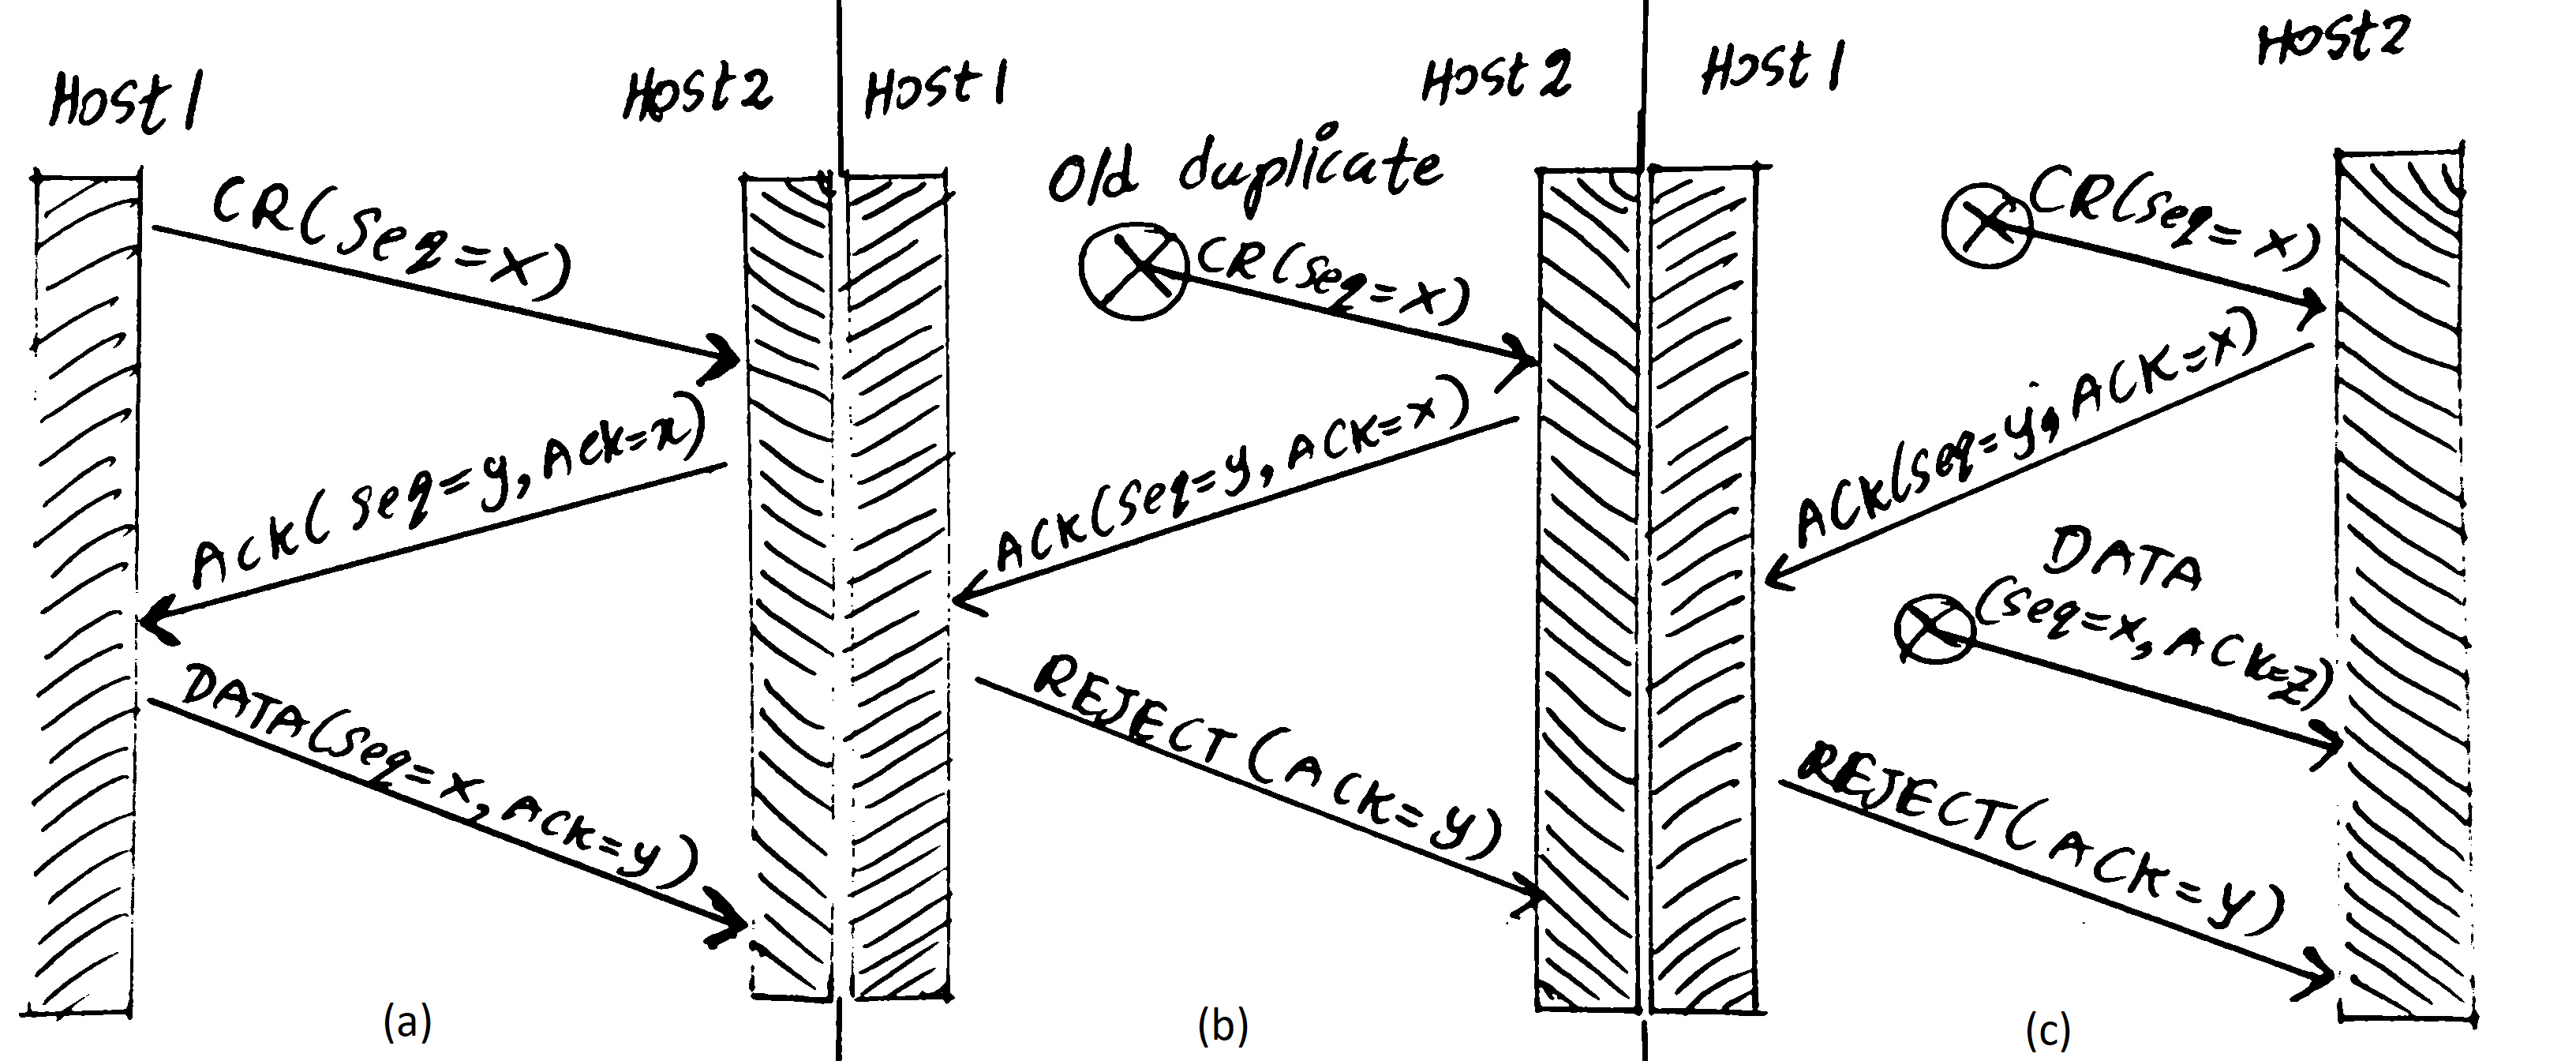
\includegraphics[scale=0.14]{figures/img100}
	\caption{\textbf{Connection establishment}: Normal case of a three-way handshake, Old CONNECTION REQUEST appearing out of nowhere and Duplicate CONNECTION REQUEST  and duplicate ACK}
\end{figure}

\subsubsection*{8.2. Connection Release}

\begin{itemize}
\item Normal case of a three-way handshake
\item Final ACK lost
\item Response lost
\item Response lost and subsequent DRs lost
\end{itemize}

\begin{figure}[H]
	\centering
	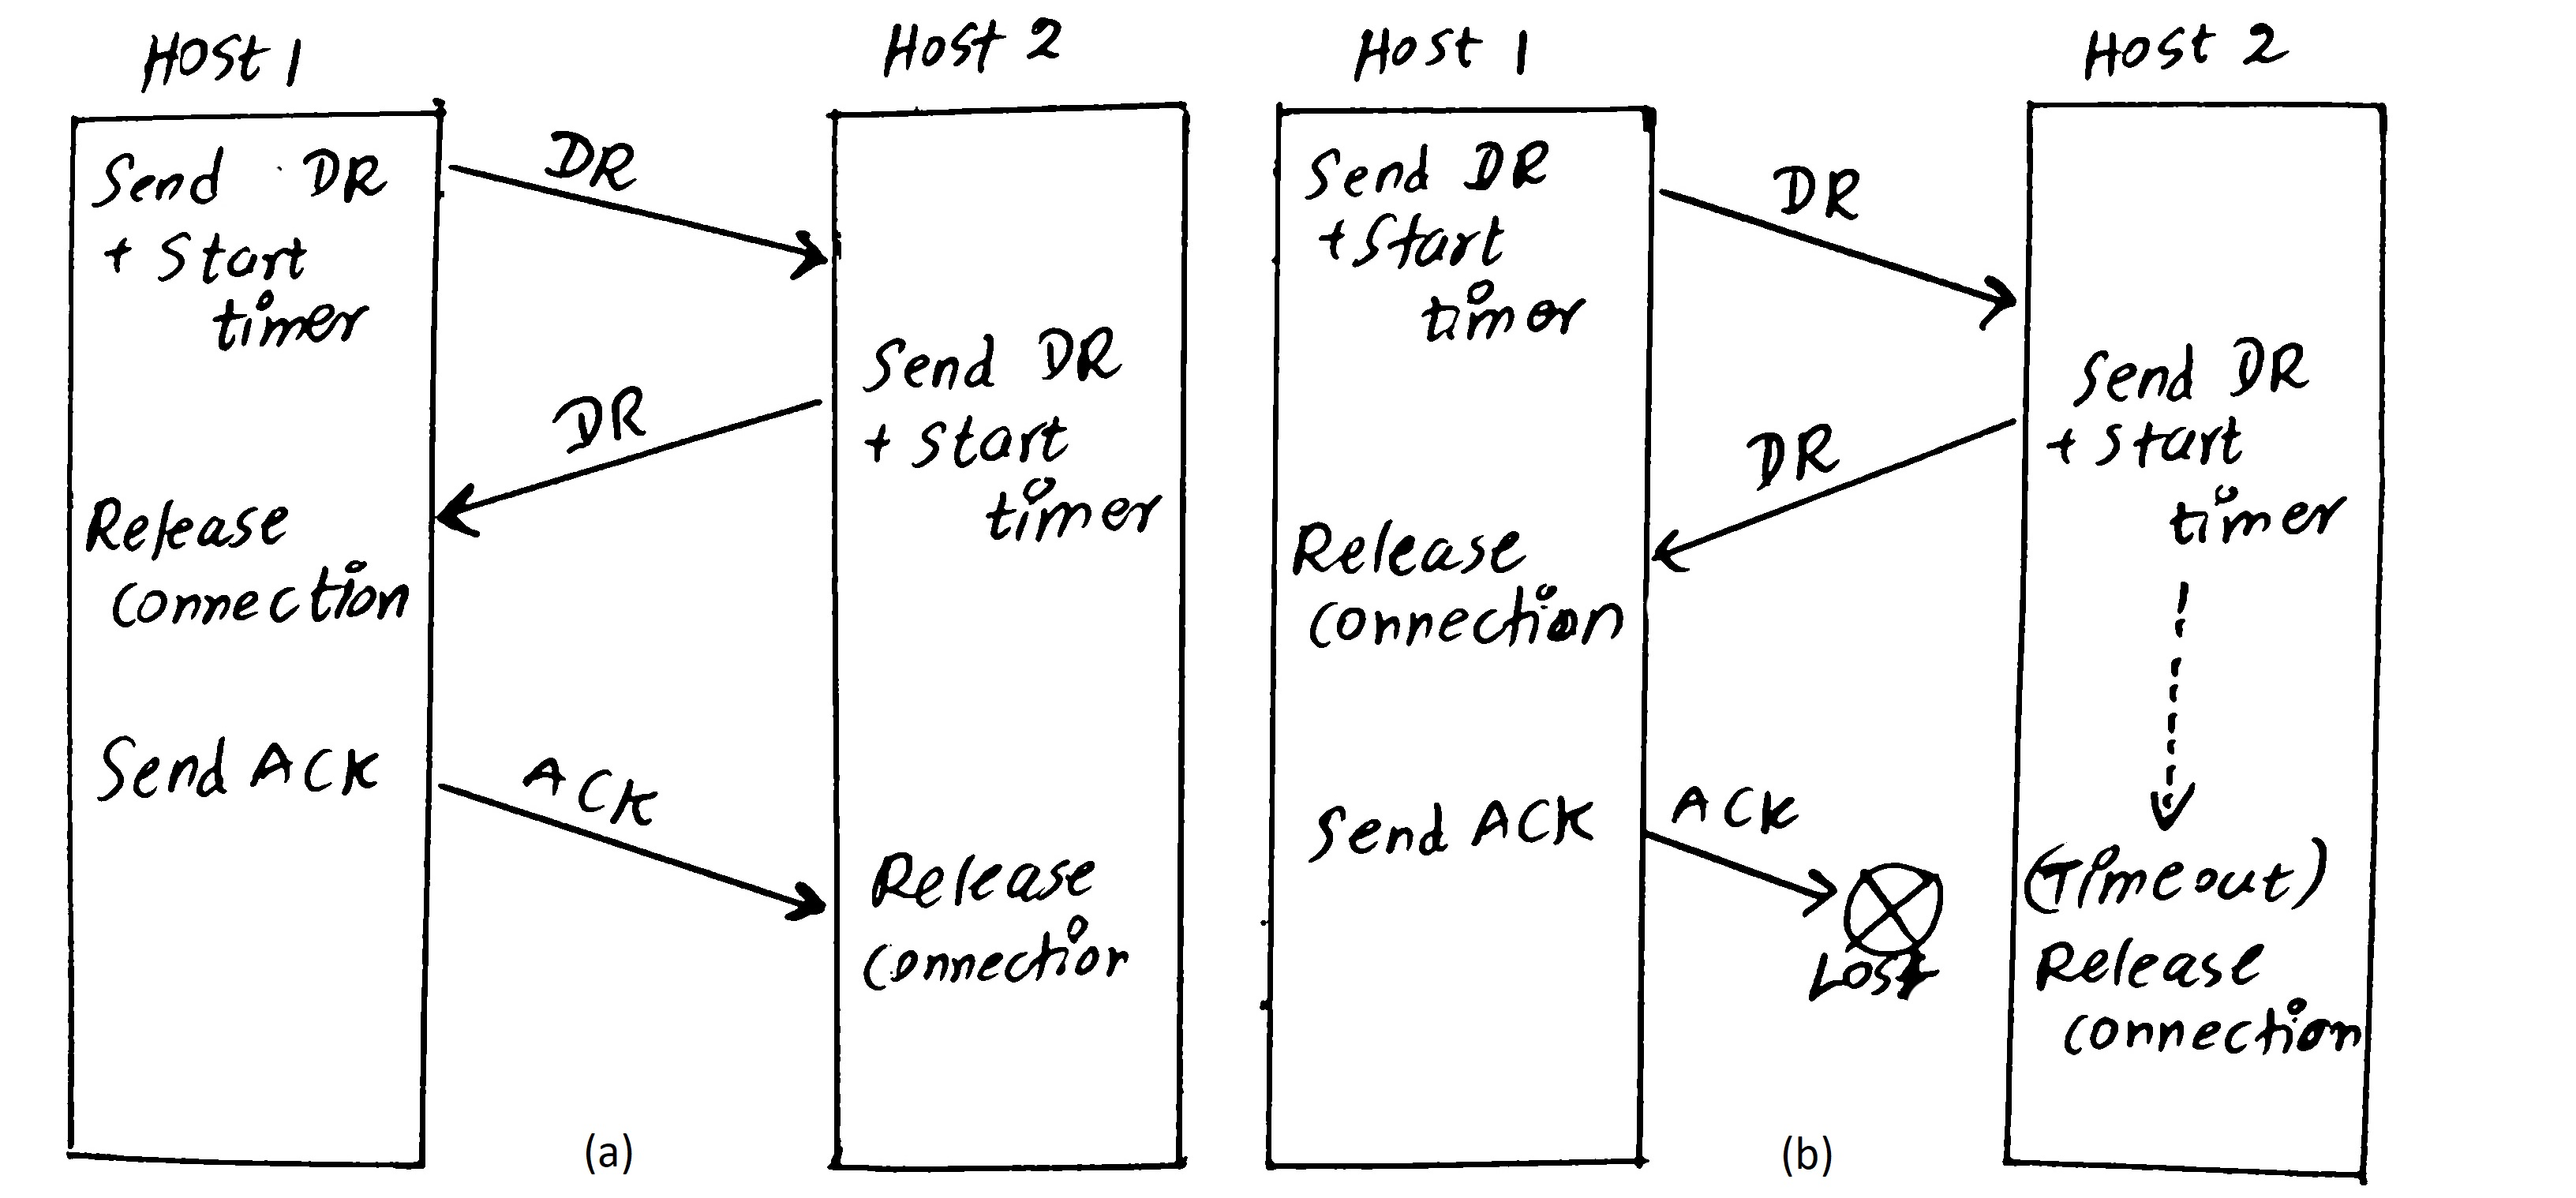
\includegraphics[scale=0.14]{figures/img101}
	\caption{\textbf{Connection Release}: Normal case of a three-way handshake and Final ACK lost}
\end{figure}

\begin{figure}[H]
	\centering
	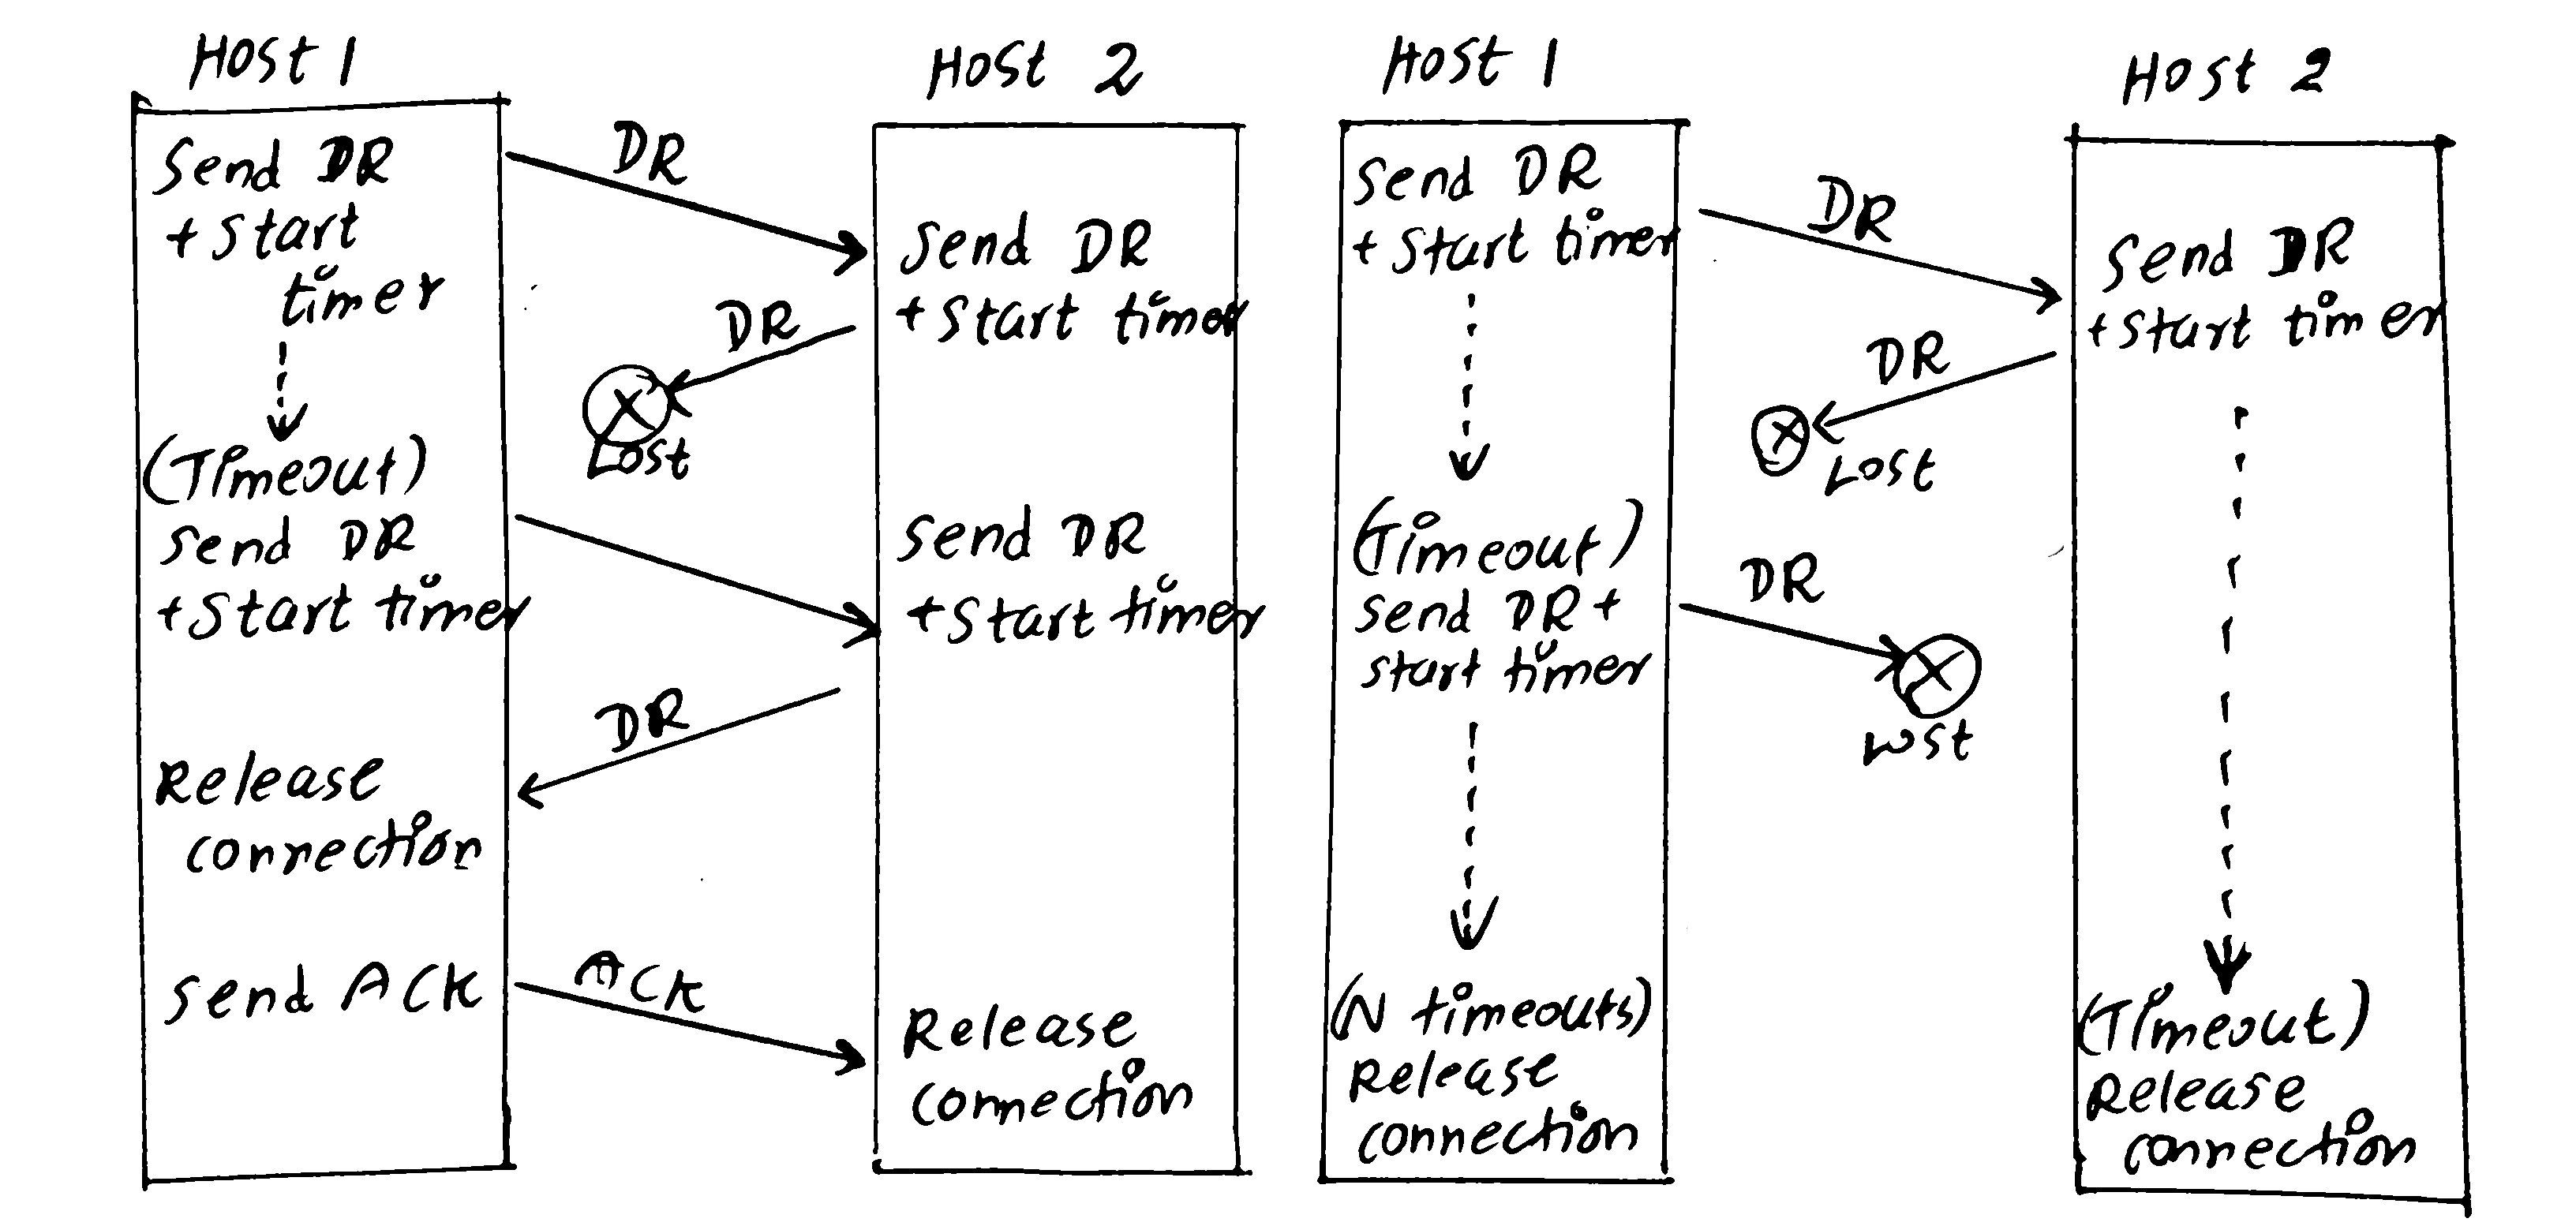
\includegraphics[scale=0.14]{figures/img102}
	\caption{\textbf{Connection Release}: Response lost and Response lost and subsequent DRs lost}
\end{figure}

\subsection*{9. What is the objective of having flow control mechanism?}

\subsection*{10. How does buffer help controlling the flow?}

\end{document}
